\documentclass[10pt]{article}

%opening
\title{Analysis of Mathematical Optimization:\\Some Classes, Problems, and Algorithms}
\author{Liam Wrubleski}
\date{April 2020}

\usepackage{amsmath}
\usepackage{amsfonts}
\usepackage{tabularx}
\usepackage{amsthm}
\usepackage{array}
\usepackage{tcolorbox}
\usepackage[backend=biber, style=ieee,sorting=none]{biblatex}
\tcbuselibrary{skins,breakable}
\usepackage[margin=1.5in]{geometry}

\let\avec\vec
\renewcommand{\vec}[1]{\mathbf{#1}}

\newcommand{\N}{\mathbb{N}}
\newcommand{\R}[1][]{ \ifx&#1& \mathbb{R} \else \mathbb{R}^{#1} \fi }
\newcommand{\Rp}[1][]{ \ifx&#1& \mathbb{R}_+ \else \mathbb{R}_+^{#1} \fi }
\newcommand{\Rsp}[1][]{ \ifx&#1& \mathbb{R}_* \else \mathbb{R}_*^{#1} \fi }
\newcommand{\isbin}{\in\{0,1\}}
\newcommand{\epi}[2][]{\ifx&#1& \mathrm{epi}#2 \else \textrm{epi}_{#1}#2 \fi }
\newcommand{\affcomb}[3][a]{#1#2 + (1-#1)#3}
\newcommand{\s}{\vec{s}}
\newcommand{\x}{\vec{x}}
%\newcommand{\vz}{\vec{0}}
\newcommand{\vz}[1]{\vec{0}_{#1}}

\renewcommand{\a}{\vec{a}}
\renewcommand{\b}{\vec{b}}
\renewcommand{\c}{\vec{c}}

\newtheorem*{definition}{Definition}
\newtheorem{theorem}{Theorem}[section]
\newtheorem{lemma}{Lemma}[section]
\newtheorem*{remark}{Remark}

\newcolumntype{L}{>{$}l<{$}}

\newenvironment{exampleblock}[1]{\tcolorbox[beamer,noparskip,breakable,title={#1}]}{\endtcolorbox}
\newenvironment{answerblock}[1]{\tcolorbox[beamer,noparskip,breakable,title={#1}]}{\endtcolorbox}

\addbibresource{senior_project_paper.bib}
\begin{document}

\maketitle

\begin{abstract}
This paper aims to provide an introduction to the field of mathematical optimization requiring little background knowledge. The high-level background and theory of mathematical optimization are discussed, with a focus on convex optimization. The theory and advantages of convex optimization are then discussed. The theory of linear programming is then discussed in detail, as is a simple implementation of Dantzig's simplex algorithm for linear programming problems, with a worked example. The theory of mixed-integer linear programming is then discussed, as well as an overview of the branch-and-cut method used to solve these problems. High-level explanations of quadratic programming, quadratically constrained quadratic programming, second-order cone programming, geometric programming, and semidefinite programming are provided, as are some areas in which each type of program is useful. Finally, in the interest of showing some items outside of convex optimization, the global black-box stochastic optimization algorithm developed by Wang et. al. is explained, although as the provided analysis in the paper is comprehensive no further analysis is provided. All material is presented either with proof where doing so provides useful insight to the beginner, or with references to external proofs where such proofs do not help with a basic understanding.
\end{abstract}

\section{Introduction}
Many problems, in mathematics and industry both, involve finding a configuration of items that minimize some cost, maximize some benefit, or both. However, beyond the simplest kinds of problems, this is often very difficult to do, especially in a computationally efficient fashion. The field of mathematical optimization aims to develop methods and algorithms for finding these optimal configurations in a relatively efficient manner.
\subsection{Notation}
Optimization programs are generally denoted in the following fashion\\
\begin{tabularx}{\textwidth}{X l L X}
	& minimize & f(\x), & \\
	& subject to & \x\in S &
\end{tabularx}
where $S$ is some set of configurations referred to as the \textbf{feasible space} or the \textbf{feasible region}, and $f$ is a function $f:S\to\R$ that determines how good a given configuration is. The problem also has a \textbf{objective sense}, which is either \textit{maximization} or \textit{minimization}. In the formulation above, the objective sense is minimization. A \textbf{solution} to this problem is generally a value $v^*\in\R\cup\{-\infty,\infty\}$ such that $v^* = \inf\{f(x)|x\in S\}$, or a configuration $x^*\in \textrm{cl}(S)$ such that $f(x^*) = \inf \{f(x)|x\in S\}$ or $\lim\limits_{x\in S\rightarrow x^*}f(x) = \inf \{f(x)|x\in S\}$. 

A problem is described as \textbf{infeasible} if $S=\emptyset$, so there are no configurations in the feasible region, or if $v^* = \infty$. A problem is described as \textbf{unbounded} if $v^* = -\infty$, so for each configuration there is some configuration that performs better. A particular configuration $x$ is \textbf{feasible} if and only if $x\in S$, and it is \textbf{infeasible otherwise}.

If the feasible space is a non-empty connected set, then the optimization problem is \textbf{continuous}. If the feasible space is disconnected, then the problem is \textbf{discrete} or \textbf{combinatorial}, and are related to \textbf{decision problems}, as the algorithm must decide which non-empty open set it should terminate in. Generally the feasible space is assumed to be a subset of $\R[n]$, as problems on other feasible spaces can be converted to problems on a subset of $\R[n]$.

\subsection{Calculus Optimization}
Upon introduction to optimization problems, many students will recall from early calculus courses some simple optimization problems solved using the first and second derivatives of a function. For example, a problem that should sound familiar to students who have taken some calculus goes as follows. 
\begin{exampleblock}{Calculus Optimization Example}
	You are on a beach next to the ocean. A lighthouse is placed in the ocean at the point (100,100), you are standing on the coastline at the point (0,0), and the coastline follows the line $y=0$. You travel at 3 m/s on the beach, and at 1 m/s in the water. What is the minimum amount of time it takes you to reach the lighthouse?
\end{exampleblock}
This is a problem that can quite easily be solved with single-variable calculus, but even slight modifications to this problem become unreasonable to attempt. For example, if the coastline just follows a sloped line instead of a horizontal line, the equations are far beyond the capabilities of an early calculus student. For more complicated problems still, they are intractable to solve by hand. For these, mathematical optimization is the best tool to use.
\subsection{No Free Lunch Theorems}
In this paper, we discuss only a few optimization algorithms. There are many different algorithms, which are used in different situations, and this is also often confusing to persons who are new to optimization. This is because all algorithms that perform well on certain problems must perform poorly on some other problems. This was shown by Wolpert and Macready in \cite{wm-nfl}, and is known as the "no free lunch" theorem, presented here without proof.
\begin{theorem}
	Given a finite set of configurations $V$ and a finite set $S\subset\R$, assume that $f:V\to S$ is chosen according to the uniform distribution over the set of all functions that map $V$ to $S$. For the problem of optimizing $f$ over $V$, no algorithm performs better on average than blind search (which at each step chooses $v\in V$ according to the uniform distribution over all elements of V that haven't been chosen before.)
\end{theorem}
This does not generally play into the considerations for optimization algorithms \cite{wdw-comp-the-nfl}, but it does formalize the idea that if an algorithm performs well on some problems then it must perform poorly on others (so that its average performance is no better than blind search). These problems are often nonsensical, but as discussed in section \ref{lp:sa}, there are algorithms with generally good performance that have poor performance on reasonable problems.

\subsection{Notes on conventions, notations, and the standard form}
As noted above, the sense of an optimization problem is either maximization or minimization. However, the convention is generally (with the exception of Linear Programming, see section \ref{lp}) to phrase problems as minimization problems. This is because the maximization problem

\begin{tabularx}{\textwidth}{X l L X}
	& maximize		& f(\x),	& \\
	& subject to	& \x\in S	&
\end{tabularx}
is equivalent\cite{boyd} to

\begin{tabularx}{\textwidth}{X l L X}
	& minimize		& -f(\x),	& \\
	& subject to	& \x\in S	&
\end{tabularx}
and having a consistent convention of minimization allows for easier algorithm development and explanation.

The feasible region may also be denoted using functions mapping $\R[n]$ to $\R$, which are required to have certain values. These are referred to as \textbf{constraint functions}, and typically take one of two forms. \textbf{Inequality constraints} are typically denoted using the indexed functions $g_i(\x) \leq 0, i=1,...,m$, while \textbf{equality constraints} are typically denoted using the indexed functions $h_i(\x)=0,i=1,...,p$. Normally, $n$ refers to the number of variables in the problem, $m$ refers to the number of inequality constraints, and $p$ refers to the number of equality constraints. When constraint functions are used, we consider the objective function $f$ to also be defined on $\R[n]$. If the maximal domain of $f$ is $\R[n]$, then $f$ is used on $\R[n]$. If the maximal domain of $f$ is $D\subset\R[n]$, then we consider optimizing $\tilde{f}:\R[r]\to\R\cup\{+\infty\}$, where 
\[
\tilde{f}(\x) = \begin{cases}+\infty, & \x\notin D\\f(\x), & \x\in D\end{cases}
\]
and the problem is also infeasible if $v^*=+\infty$. Problems phrased using constraint functions as follows are in \textbf{standard form}\cite{boyd}
\\
\begin{tabularx}{\textwidth}{X l L L X}
	& minimize		& f(\x) 			& 			& \\
	& subject to	& g_i(\x) \leq 0,	& i=1,...,m	& \\
	&				& h_i(\x) = 0,		& i=1,...,p &
\end{tabularx}
The feasible region is then the set $S = \{\x\in\R[n]|\forall i=1,...,m, g_i(\x)\leq0, \forall i=1,...,p, h_i(\x)=0\}$.\\

Although the feasible region does not by the definition above need to include its boundary, for continuous objective functions bounded on the closure of $S$, $v^*=\inf \{f(x)|x\in \textrm{cl}(S)\}$ is equivalent to $v^* = \min \{f(x)|x\in \textrm{cl}(S)\}$, so for the sake of convenience in this paper we assume $S$ contains its boundary (denoted $\partial S$) and use $\min$.

\section{Convex Optimization}
\subsection{Introduction}
Convex optimization encompasses many different problems, and many different kinds of problems. Further sections analyze particular subclasses of convex optimization, but the analysis would be incomplete without first discussing convex optimization as a general field, so here follows an extremely simplified overview of convex optimization.
\subsection{Theory}
The foundation of convex optimization is convex sets and convex functions, so below are given the definitions of convex sets and functions. 
\begin{definition}[Convex Set]
	A set $S\subseteq\R[n]$ is \textbf{convex} if and only if for any two points $\x_1, \x_2\in S$ and any $a\in[0,1]$, $\affcomb{\x_1}{\x_2}\in S$. \cite{boyd}
\end{definition}
\begin{definition}[Epigraph]
	The \textbf{epigraph} of a function $f:S\to\R, S\subseteq\R[n]$ is the set $\epi{f}=\{(\x,v)|\x\in S, v \geq f(\x)\}\subset\R[n+1]$. \cite{boyd}
\end{definition}
\begin{definition}[Convex Function]
	A \textbf{convex function} is a function $f:S\to\R$, where $S$ is a convex set, such that $\epi{f}$ is a convex set. Equivalently, $f$ is a convex function if and only if for any two points $\x_1,\x_2\in S$ and any $a\in[0,1]$, $f(\affcomb{\x_1}{\x_2})\leq\affcomb{f(\x_1)}{f(\x_1)}$.\cite{boyd}
\end{definition}
\begin{definition}[Concave Function]
	A \textbf{concave function} is a function $f$ such that $-f$ is a convex function.\cite{boyd}
\end{definition}

\begin{theorem}
	The intersection of two convex sets is a convex set.
\end{theorem} 
\begin{proof}
	Take any two convex sets $C_1, C_2\subseteq\R[n]$. Then let $\vec{x}_1, \vec{x}_2\in C_1\cap C_2, a\in[0,1]$.  Then $\affcomb{\vec{x}_1}{\vec{x}_2}\in C_1$, as $\vec{x}_1, \vec{x}_2\in C_1$ by construction and $C_1$ is convex. Similarly, $\affcomb{\vec{x}_1}{\vec{x}_2}\in C_2$, so $\affcomb{\vec{x}_1}{\vec{x}_2}\in C_1\cap C_2$, so $C_1\cap C_2$ is convex.
\end{proof}

Equipped with these definitions, a convex optimization problem may be defined as follows:
\begin{definition}[Convex Optimization Problem]
	A \textbf{convex optimization problem} is an optimization problem with feasible region $S$ and objective function $f$ of the form \\
	\begin{tabularx}{\textwidth}{X l l X}
		& minimize & $f(\x),$ & \\
		& subject to & $\x\in S$ &
	\end{tabularx}
	where $S$ is a convex set, and $f$ is a convex function.
\end{definition}
\begin{remark}
	In order to perform convex optimization with the objective sense being maximization, $-f$ must be convex, so $f$ must be concave.
\end{remark}
To explain why convex optimization is especially useful, several more definitions are required.
\begin{definition}[Local Optimum]
	A point $\x^*\in\bar{S}$ is a \textbf{local optimum} for the optimization problem $(S,f)$ if $\exists\varepsilon>0:\forall \x\in \bar{S}:\lVert \x-\x^*\rVert < \varepsilon\implies f(\x)\geq f(\x^*)$.
\end{definition}
\begin{definition}[Global Optimum]
	A point $\x^*$ is a \textbf{global optimum} for the optimization problem with feasible region $S$ and objective function $f$ if $\forall \x\in S, f(\x)\geq f(\x^*)$.
\end{definition}
\begin{theorem}
	Any local optimum to a convex optimization problem is a global optimum to that optimization problem.
\end{theorem}
\begin{proof}
	Suppose $(S,f)$ describes a convex optimization problem, and suppose for the sake of contradiction that $f$ has a local optimum $\x_0\in\bar{S}$ which is not a global optimum of $f$. Then there exists some point $\x^*$ such that $f(\x^*) < f(\x_0)$. As $\x_0$ is a local minimum of this problem, there exists $\varepsilon>0$ such that $\forall \x\in \bar{S}:\lVert \x-\x_0\rVert < \varepsilon\implies f(\x)\geq f(\x_0)$. Take such an epsilon, then consider $a = \frac{\varepsilon}{2\lVert\x^*-\x_0\rVert}$ and $\x_1=\affcomb{\x^*}{\x_0}$. As $S$ is a convex set, we know $x_1\in S$. This gives that $\lVert\x_1-\x_0\rVert = \lVert(\affcomb{\x^*}{\x_0}) - \x_0\rVert = \lVert a(\x^*-\x_0) + \x_0 - \x_0\lVert = \frac{\varepsilon\lVert\x^*-\x_0\rVert}{2\lVert\x^*-\x_0\rVert} = \frac{\varepsilon}{2} < \varepsilon$, so $f(\x_1) \geq f(\x_0)$. However, from the definition of a convex function, we know that $f(\x_1) = f(\affcomb{\x^*}{\x_0}) \leq\affcomb{f(\x^*)}{f(\x_0)}<\affcomb{f(\x_0)}{f(\x_0)}=f(\x_0)$. So we have that $f(\x_1) \geq f(\x_0)$ and $f(\x_1) < f(\x_0)$, which is a contradiction. 
\end{proof}
This property of convex optimization problems makes them very attractive, as it is only required to find a single local minimum in order to globally optimize the function.

As with mathematical optimization in general, the feasible space is usually expressed in standard form using constraint functions\cite{boyd}. For convex optimization problems, the standard form looks as follows:
\\
\begin{tabularx}{\textwidth}{X l L L X}
	& minimize		& f(\x) 			& 			& \\
	& subject to	& g_i(\x) \leq 0,	& i=1,...,m	& \\
	&				& h_i(\x) = 0,		& i=1,...,p &
\end{tabularx}
where $f$ is a convex function, $g_i$ are all convex functions, and $h_i$ are all affine functions (see section \ref{lp}). This makes the feasible space \[
S = \left(\bigcap\limits_{i=0}^{m} \epi{g_i}\right)\cap\left(\bigcap\limits_{i=0}^{p} \{(\x,0)\in\R[n+1]|h_i(\x)=0\}\right)\cap\{(\x,v)\in\R[n+1]|v\leq 0\}
\]
As this is the intersection of convex spaces, it is also convex.
\section{Linear Programming}
\label{lp}
\subsection{Introduction}
Linear programming is a relatively simple subclass of convex optimization, limiting the ways in which the feasible space can be defined, and which objective functions are permitted to be used. This makes them much easier to solve, as it is possible to take advantage of structure in the problem, but it also limits the real-world problems that can be described. For example, linear programming cannot use Euclidean distance between points as a constraint, which means that it cannot be used to solve problems involving the placement of items. 

It should be noted that the word programming in an optimization context does not relate to the idea of computer programming, but rather exists for historical reasons. It largely derives from the work of George B. Dantzig, who developed the simplex algorithm for solving linear programming problems, as he was working for the United States military, which used the term "program" to describe proposed schedules \cite{dantzig}. As his work was seminal in the field, the terminology has become standard.
\begin{definition}[Halfspace]
	A \textbf{halfspace} $H_{\vec{v},b}\subset\R[n]$ is the union of all points on one side of the $n-1$ dimensional hyperplane defined by $\vec{v}\in\R[n]\setminus\vz[n], b\in\R$ and all points in that hyperplane: for some vector $\vec{v}\in\R[n]\setminus\vz[n], b\in\R, S = {\x\in\R[n] | \vec{v}\cdot\x \geq b}$.
\end{definition}
\begin{theorem}
	All halfspaces are convex.
\end{theorem}
\begin{proof}
	Take any halfspace $H_{\vec{v},b}\subset\R[n]$. Take any $\x_1, \x_2\in H_{\vec{v},b}$. Then for any $a\in[0,1], (\affcomb{\x_1}{\x_2})\cdot\vec{v} = \affcomb{\x_1\cdot\vec{v}}{\x_2\cdot\vec{v}} \geq \affcomb{b}{b} = b$, so we have that $\affcomb{\x_1}{\x_2}\in H_{\vec{v},b}$, so $H_{\vec{v},b}$ is convex.
\end{proof}
\begin{remark}
	An alternative definition of a convex set in $\R[n]$ is the intersection of (potentially infinitely many) halfspaces in $\R[n]$.
\end{remark}
Linear programming is optimization of a linear objective function in $\R[n]$ where the feasible space is the intersection of finitely many halfspaces in $\R[n]$. Phrased equivalently, the feasible space is a (possibly unbounded) convex polytope in $n$ dimensions, with faces defined by the bounding hyperplanes of the halfspaces. However, this definition is difficult to use in the construction of an algorithm, so we typically write an LP problem as a constrained problem in $\R[n]$, where the constraint functions are all affine.
\begin{definition}[Affine function]
An affine function is a function $f:\R[n]\to\R$ of the form $f(\x) = \c^T\x + b$, for some $\c\in\R[n], b\in\R$. In other words, an affine function is a linear function plus a constant.
\end{definition}
\subsection{Theory}
Transforming this definition to the standard form is straightforward. Note that here the convention is to maximize the objective function, which is historical in nature and simplifies some notation later, but is equivalent to a minimization problem as stated earlier.\\
\begin{tabularx}{\textwidth}{X l l l X}
	& maximize		& $f(\x) = \c ^T\x$						& 				& \\
	& subject to	& $g_i(\x) = \a _i^T\x - b_i \leq 0,$	& $i=1,...,m$	& \\
	& 				& $h_i(\x) = \c _i^T\x - d_i = 0,$		& $i=1,...,p$
\end{tabularx}
While this is in standard form as described above, for linear programming problems there is a slight variation to the standard form that is typically used, called the \textbf{canonical form} of the LP problem. This is obtained from the standard form using transformations discussed in section \ref{lp:sa}, and appears as follows:\\
\begin{tabularx}{\textwidth}{X l l X}
	& maximize		& $\c^T\x$ & \\
	& subject to	& $A\x\leq \b $ & \\
	& 				& $\x\geq\vz{}$ & 
\end{tabularx}
where the inequality signs here are comparing vectors elementwise.
\subsection{Simplex Algorithm}
\label{lp:sa}
The simplex algorithm was developed by George B. Dantzig. It is an algorithm for solving LP problems, and has been shown to be fairly efficient in real-world applications, and on random problems. Its worst case performance was shown by Klee and Minty to be exponential time in the number of dimensions, but on real-world problems and in general, it tends to be polynomial time in the number of dimensions. This has been shown in several fashions, which are unfortunately beyond the scope of this analysis. We will explore the specific results obtained from these sources, though, after analyzing the algorithm itself.

The simplex algorithm accepts linear programming problems in canonical form.\cite{murty}\\
\begin{tabularx}{\textwidth}{X l l X}
	& maximize		& $\c^T\x$ & \\
	& subject to	& $A\x\leq \b$ & \\
	& 				& $\x\geq\vz{n}$ & 
\end{tabularx}
If the problem is not in canonical form, it is transformed into canonical form as follows.\cite{murty} If there are any equality constraints $h(\x)=0$, they are each transformed into two inequality constraints $h(\x)\leq 0, -h(\x)\leq 0$. If any variable $x_i$ is unbounded, it is replaced with two variables $x_i^+, x_i^-\geq 0$, substituting $x_i = x_i^+ - x_i^-$ in each of the other functions. If any variable $x_i$ is not bounded from below, but it is bounded from above (i.e. $x_i \leq b_i$), then substitute $x_i = b_i - y_i$, with $y_i\geq 0$. Finally, if any variable $x_i$ is bounded from below, but not by 0 (i.e. $x_i \geq k_i \neq 0$), then substitute $x_i = y_i+k_i$, with $y_i\geq 0$.

It is also worth discussing the matrix inequality. If we consider the original inequality constraints $g_i(\x) = \a_i^T\x - b_i$, then we construct the matrix $A$ and the vector $\b$ from these constraints by setting the $i$-th row of $A$ to be $\a_i^T$, and the $i$-th element of $\b$ to be $b_i$, so that using the elementwise inequality $A\x-b\leq\vz{m}$ encapsulates the same information as the original inequality constraints. Finally, we rearrange to obtain $A\x\leq\b$.

When given an LP problem in canonical form, the simplex algorithm first begins by taking each inequality constraint encapsulated in the matrix $A$ and the vector $\b$, and converting it to an equality constraint using a \textbf{slack variable}. This variable does not appear in the objective function, and only appears in one of the inequality constraints. For the inequality constraint $g_i(\x) = \a_i^T\x - b_i\leq 0$, we add the slack variable $s_i$ so that we obtain $\a_i^T-b_i + s_i = 0, s_i\geq 0$. 
\begin{remark}
	It may seem counter intuitive to convert each equality constraint to two inequality constraints, and then to convert each inequality constraint to an equality constraint. Indeed, as touched on in section \ref{lp:sa-phaseone}, the initial equality constraints may be used. Here we perform this conversion so that we only have inequality constraints, which simplifies our explanation. For further information, see section \ref{lp:sa-phaseone}.
\end{remark}
Using these slack variables, the constraints then become $A\x + \s = \b, \x\geq \vz{n}, \s\geq \vz{m}$, while the objective function takes the form $\c^T\x + \vz{m}^T\s$. The algorithm then arranges the problem into a particular kind of matrix called a \textbf{tableau}:
\begin{align}
\label{lp:sa-tableau}
\begin{bmatrix}
1 & \c^T & \vz{m}^T & 0\\
0 & A & I_m & \b. 
\end{bmatrix}
\end{align}
\begin{remark}
	This method of construction of the tableau implicitly assumes that $\x=\vz{n}$ is a feasible solution, which is not necessarily true. If this does not hold, then the initial tableau must be constructed in an alternative fashion, which is to run the simplex algorithm on a modified version of the problem. This is explained in section \ref{lp:sa-phaseone}.
\end{remark}
The algorithm then performs operations called \textbf{pivots} on this tableau to obtain possible solutions\cite{dantzig-intro}. At any given point during the operation of the algorithm, the variables corresponding to columns of the matrix which are columns of the $m+1$ dimensional identity matrix are called \textbf{basic variables}, and all other variables are \textbf{nonbasic variables}. All nonbasic variables are 0, and basic variables take on values from the rightmost column (i.e. if the column corresponding to $x_i$ has zeroes in every row except row $j>1$, and has value $1$ in row $j$, then $x_i$ = $b_{j-1}$). The first column corresponds to the value of the objective function $Z = -f(\x)$, or $Z+f(\x) = 0$.
\subsubsection{Pivot Operations}
\label{lp:sa-pivotops}
With an understanding of the current solution given a configuration of the tableau, we can now explain the pivot operation. First, recall from the introduction of LPs that the feasible space is a convex polytope. The method of construction of the initial tableau ensures that the initial solution always sits on a vertex of this polytope, and pivot operations move the algorithm from one feasible vertex of the polytope to another. This algorithm works because if the feasible space is not empty, and the objective function has a maximum on any point in the feasible region, then there exists at least one vertex of the polytope at which the objective function takes on its maximum. 
\begin{lemma}
	\label{lp:sa-pivotops-l1}
	If a nonzero linear function $f:\R[n]\to\R$ takes on a maximum $M$ at a point $\x^*$ in a space $S$, then $\x\in\partial S$.
\end{lemma}
\begin{proof}
	Suppose $f(\x^*) = \max_{\x\in S}\{f(\x)\}$ (i.e. $f$ takes on its maximum over $S$ at $\x^*$). Note that as $f$ is linear and nonzero, there exists some $\c\in\R[n]\setminus\vz{n}$ such that $f(\x) = \c^T\x$. Then for any $\varepsilon>0, f(\x^* + \frac{\varepsilon}{\lVert\c\rVert}\c) = \c^T(\x^*+\frac{\varepsilon}{\lVert\c\rVert}\c) = \c^T\x^* + \frac{\varepsilon}{\lVert\c\rVert}\lVert\c\rVert^2 = \c^T\x^*+\varepsilon\lVert\c\rVert > \c^T\x^*$, so we have that $\x^*+\frac{\varepsilon}{\lVert\c\rVert}\c\notin S$, as $\x^*$ is the maximum over $S$. However, $\x^*+\frac{\varepsilon}{\lVert\c\rVert}\c\in N_\varepsilon(\x^*)$, so $\forall\varepsilon>0,\exists\x\in N_\varepsilon(\x^*): \x\notin S$, and $\x^*\in S$, so we have that $\x^*$ is a boundary point of $S$, so $\x^*\in\partial S$.  
\end{proof}
\begin{theorem}[Fundamental theorem of linear programming]
	If a linear programming problem in canonical form with objective function $f$ has a maximum over its feasible region, then $f$ takes on that maximum for at least one vertex of the feasible region.
\end{theorem}
\begin{proof}
	\label{lp:sa-pivotops-t1}
	If the objective function $f(\x) = 0$, then the function takes on its maximum at all points in the feasible region. As the feasible region is a nonempty polytope, it has at least one vertex, so $f$ takes on its maximum at at least one vertex of the feasible region.
	
	If the objective function $f(\x) = \c^T\x, \c\neq\vz{n}$, then by lemma \ref{lp:sa-pivotops-l1}, we know that $\exists\x_0$ in the boundary of the feasible region that maximizes $f$. Then $\x_0$ must lie in some "hyperface" of the feasible region (i.e. in 3 dimensions, it can lie in a 0-face (vertex), 1-face (edge), or 2-face (face)). Let $F$ represent the lowest dimensional face of the feasible region that $\x_0$ lies in, and $j$ represent the dimension of $F$. If $j$ is 0, then $\x_0$ is a vertex of the feasible region. Otherwise, if $j>0$, then there exist $j$ orthogonal vectors $\vec{v}_i$ such that for each of these vectors, there exists some $\varepsilon_i>0: 0<\delta<\varepsilon\implies \x_0 + \delta\vec{v}_i\in F\land\x_0 - \delta\vec{v}_i\in F$. As $\x_0$ maximizes $f$ over the entire feasible region, we must then have that $\c^T\vec{v}_i = 0$ for each $\vec{v}_i$, which implies that $F$ lies entirely in the hyperplane $\{x\in\R[n]:\c^T\x=\c^T\x_0\}$. Then, as $F$ has at least one vertex, there is at least one vertex $\x^*$ with $f(\x^*)=f(\x_0)$.
\end{proof}
At any given step, if the slack variable associated with an inequality is a nonbasic variable, then that inequality is currently true as an equality. Additionally, the values of the first row of the tableau are the partial derivatives of the objective function with respect to each variable. A pivot operation takes a nonbasic variable (called the \textbf{entering variable}) and makes it into a basic variable, and simultaneously takes a basic variable (called the \textbf{leaving variable}) and makes it into a nonbasic variable. It proceeds as follows:
\begin{enumerate}
	\item If all entries in the first row are negative, the current solution is optimal, so return $Z$.
	\item Otherwise, take $c$ to be the leftmost column with a positive element in the first row \cite{bland} (this is the entering variable choice rule, others can be used).
	\item If all entries in column $c$, other than the first one, are negative, the problem is unbounded, so return $+\infty$.
	\item Otherwise, let $a_{rc}$ denote the element in row $r$ of column $c$, and $b_r$ denote the element in row $r$ of the rightmost column of the tableau.
	\item Take $r$ to be the row that minimizes $b_r/a_{rc}$. If multiple rows have the same value, take the first one whose basic variable is the furthest to the left \cite{bland} (this is the dropping variable choice rule, others can be used).
	\item Divide row $r$ by $a_{rc}$, then add multiples of row $r$ to each other row in the tableau such that column $c$ is a column of the identity matrix.
\end{enumerate}
The entering variable is the variable associated with column $c$, and the leaving variable is the basic variable that previously had a 1 in row $r$. By selecting the row which minimizes the value of $b_r/a_{rc}$, when the row operations are performed to make column $c$ into a column of the identity matrix, we ensure that the values in the rightmost column always stay positive, ensuring that the resulting solution is still feasible. Another interpretation is that when the variable enters, it goes from 0 to whichever constraint is most tightly bounding the value of that variable, which ensures that the resulting solution is feasible. \cite{dantzig}
\subsubsection{Initial Tableau and Solution}
\label{lp:sa-phaseone}
The problem arises of how to find an initially feasible vertex of the polytope. If the origin is a feasible point, then it is a feasible vertex, but if the origin is not feasible then a different method of finding a feasible vertex is required. This method also allows for the direct usage of equality constraints. Suppose we are given a linear programming problem for which the origin is not a feasible point after all of the aforementioned transformations, or which is not in canonical form
\begin{tabularx}{\textwidth}{X l l X}
	& maximize		& $\c^T\x$ & \\
	& subject to	& $A_s\x\leq \b_s$ & \\
	& 				& $A_v\x\leq \b_v$ & \\
	& 				& $C\x = \vec{d}$ & \\
	& 				& $\x\geq\vz{n}$ & 
\end{tabularx}
where $A_s, \b_s$ correspond to the $m$ inequality constraints which are satisfied at the origin, $A_v, \b_v$ correspond to the $p$ inequality constraints
which are not satisfied at the origin, and $C, d$ correspond to $q$ equality constraints. Then construct the non-canonical tableau 
\begin{align*}
\begin{bmatrix}
1		& \c^T	& \vz{m}^T	&\vz{p}^T	& 0\\
\vz{m}	& A_s	& I_m 		& \vz{p,p}	& \b_s\\
\vz{p}	& A_v	& \vz{m,m}	& I_p		& \b_v\\
\vz{q}	& C		& \vz{m,m}	& \vz{p,p}	& d
\end{bmatrix}
\end{align*}
This tableau does not correspond to a valid solution to the linear programming problem, as all the inequality constraints which are violated at the origin are violated, and no attempt has been made to address the equality constraints. The first step in solving these issues is that if any entries in the rightmost column are negative, that entire row is negated (this is valid as each row corresponds to an equality). Then, a new, canonical tableau is constructed by adding new virtual artificial variables, and adding a new objective function, which is the sum of these virtual variables. We attempt to minimize this new objective function, so when adding it to the tablea 	u it is negated. Finally, in order to get the tableau to be canonical, each of the artificial variables is made into a basic variable, by adding its corresponding row to the first row (this is not shown in the tableau below). 
\begin{align*}
\begin{bmatrix}
1	& 0 		& \vz{n}^T	& \vz{m}^T	& \vz{p}^T	& -\vec{1}_p^T	& -\vec{1}_q^T	& 0\\
0	& 1			& \c^T		& \vz{m}^T	& \vz{p}^T	& \vz{p}^T		& \vz{q}^T		& 0\\
0	& \vz{m}	& A_s		& I_m 		& \vz{p,p}	& \vz{p,p}		& \vz{q,q}		& \b_s\\
0	& \vz{p}	& A_v		& \vz{m,m}	& I_p		& I_p			& \vz{q,q}		& \b_v\\
0	& \vz{q}	& C			& \vz{m,m}	& \vz{p,p}	& \vz{p,p}		& I_q			& d
\end{bmatrix}
\end{align*}
The simplex method is then run on this canonical tableau, and if this returns a minimum value of 0 then the internally stored tableau is a canonical representation of the original LP problem. Otherwise, if this returns a positive minimum value, then the original LP problem is infeasible (i.e. the feasible space is empty). This is referred to as the $Phase 1$ computation.\cite{murty}
\subsubsection{Worked Example}
The above information is difficult to understand without a particular reference, so a simple worked example is presented here. Consider the following problem: \\
\begin{exampleblock}{Linear Programming Example Problem}
	A farmer has 10 square kilometers of land on which she can grow wheat and barley, in any positive combination of the two. She also has 17 kg of fertilizer, and 13 kg of pesticide. For each square kilometer of wheat she grows, she needs 2 kg of fertilizer and 2 kg of pesticide, and she can sell the wheat for \$6000 of profit per square kilometer. For each square kilometer of barley she grows, she needs 3 kg of fertilizer, and 1 kg of pesticide, and she can sell the barley for \$5000 of profit per square kilometer. Finally, suppose she needs to plant at least 1 square kilometer of crops, regardless of any other consideration, in order to meet her quota. How should she plant these crops to maximize her profit?
\end{exampleblock}
\begin{answerblock}{Linear Programming Example Evaluation}
	This problem is obviously contrived, and can be solved quite simply using far simpler methods. However, here we go through the entire simplex method for the purpose of illustration. First, convert the constraints set using words to inequalities, letting $x$ represent the amount of land allocated to wheat in km$^2$, and $y$ represent the amount of land allocated to barley in km$^2$. Then we obtain the following constraints:
	\begin{enumerate}
		\item The total amount of land available is 10 square kilometers $\implies x+y\leq 10$.
		\item The total amount of fertilizer is 17 kilograms $\implies 2x+3y \leq 17$.
		\item The total amount of pesticide is 13 kilograms $\implies 2x + y\leq 13$.
		\item She needs to plant at least 1 km$^2$ of crops $\implies x+y \geq 1$.
		\item She wants to maximize her profit (in thousands of dollars) $\implies \textrm{maximize }6x+5y$.
	\end{enumerate}
	Here we see the feasible space for this problem pictured, where the blue region is the feasible space, the blue line is its boundary, and the grey lines are the inequalities. The red arrow is the direction of maximization.
	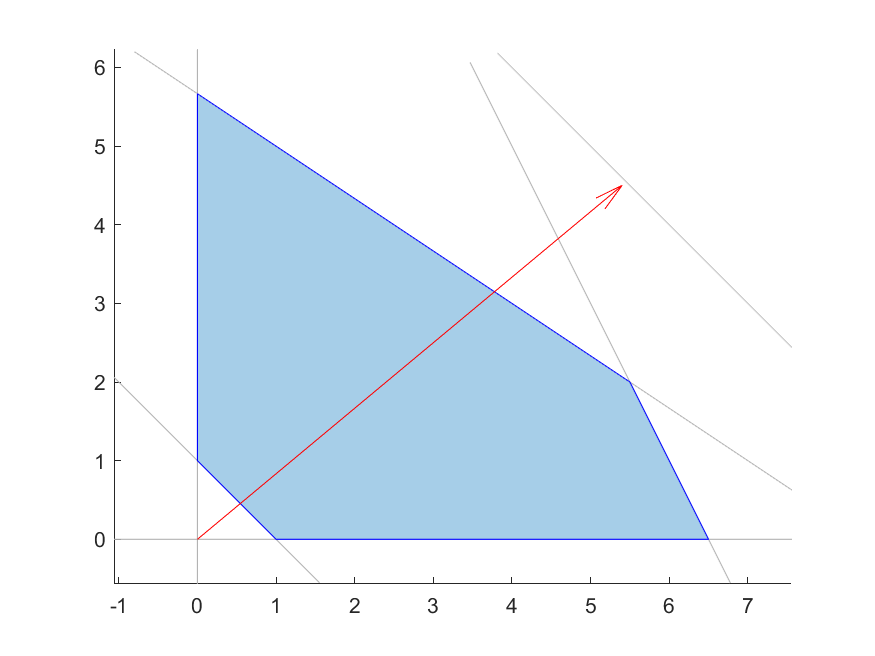
\includegraphics[width=\textwidth]{images/paper_simplex_problem.png}
	Adding slack variables and rearranging, we obtain the equalities
	\begin{enumerate}
		\item $x + y + s_1 = 10$
		\item $2x + 3y + s_2 = 17$
		\item $2x + y + s_3 = 13$
		\item $-x-y+s_4 = -1$
	\end{enumerate}
	We can then arrange these equalities into a tableau as described above. Note that here we include the variable names as the first row of the matrix, but these are not actual elements of the matrix. They are listed only to help the reader keep track of variables through different iterations. Not also that when a pivot operation is performed, the entering and leaving elements are bolded. This does not, in this context, correspond to vectors.
	\begin{minipage}{0.6\textwidth}
		\begin{align*}
		\begin{bmatrix}
		Z	& x		& y		& s_1	& s_2	& s_3	& s_4	& b \\
		1	& 6		& 5		& 0		& 0		& 0		& 0		& 0 \\
		0	& 1		& 1		& 1		& 0		& 0		& 0		& 10 \\
		0	& 2		& 3		& 0		& 1		& 0		& 0		& 17 \\
		0	& 2		& 1		& 0		& 0		& 1		& 0		& 13 \\
		0	& -1	& -1	& 0		& 0		& 0		& 1		& -1
		\end{bmatrix}
		\end{align*}
	\end{minipage} \hfill
	\begin{minipage}{0.35\textwidth}
		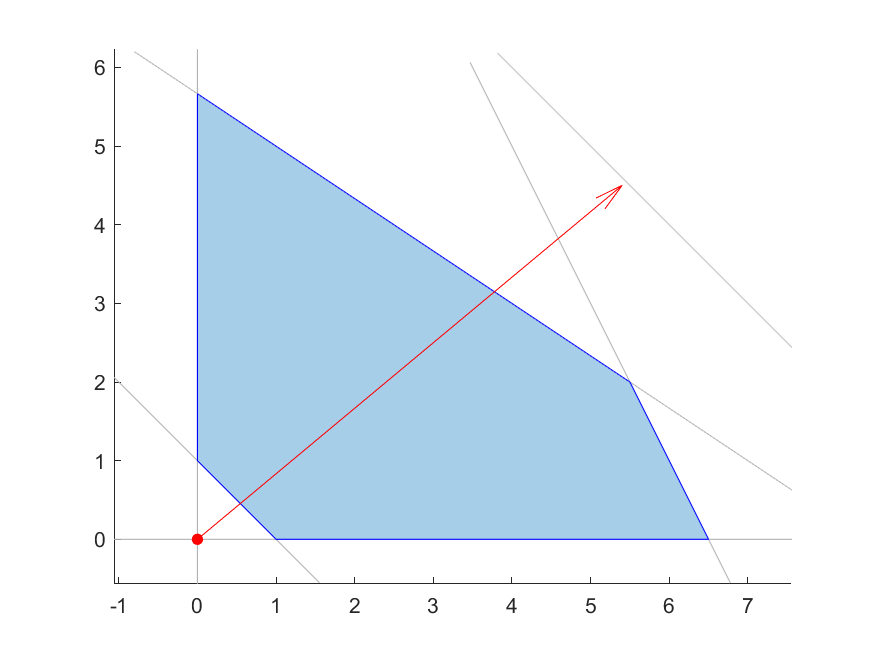
\includegraphics[width = \textwidth]{images/paper_simplex_point_inv.png}
	\end{minipage}

	\vspace{6pt}
	While this tableau is a canonical tableau, it does not correspond to a valid solution, as we have $s_4$ as a basic variable, with a value of $-1$, so this is not a feasible configuration. We can see this in the image, as the red point representing our current solution does not lie within the feasible region. Although it is trivial to guess where we could place the starting point, we go through the Phase 1 computation for the sake of illustration. We begin by negating the last row, then adding an artificial variable $u$ to it, giving us the following canonical tableau, upon which we begin to execute the simplex method
	\begin{align*}
	&\begin{bmatrix}
	W	& Z	& x				& y	& s_1	& s_2	& s_3	& s_4	& u	& b \\
	1	& 0	& \textbf{1}	& 1	& 0		& 0		& 0		& -1	& 0	& 1 \\
	0	& 1	& 6				& 5	& 0		& 0 	& 0 	& 0		& 0	& 0 \\
	0	& 0	& 1 			& 1 & 1 	& 0 	& 0 	& 0		& 0	& 10 \\
	0	& 0	& 2 			& 3 & 0 	& 1 	& 0 	& 0		& 0	& 17 \\
	0	& 0	& 2 			& 1 & 0 	& 0 	& 1 	& 0		& 0	& 13 \\
	0	& 0	& \textbf{1}	& 1 & 0 	& 0 	& 0 	& -1	& 1	& 1
	\end{bmatrix}\\
	\rightarrow
	&\begin{bmatrix}
	W	& Z	& x	& y		& s_1	& s_2	& s_3	& s_4	& u		& b \\
	1	& 0	& 0	& 0		& 0		& 0		& 0		& 0		& -1	& 0 \\
	0	& 1	& 0	& -1	& 0		& 0 	& 0 	& 6		& -6	& -6 \\
	0	& 0	& 0 & 0		& 1 	& 0 	& 0 	& 1		& -1	& 9 \\
	0	& 0	& 0 & 1		& 0 	& 1 	& 0 	& 2		& -2	& 15 \\
	0	& 0	& 0	& -1	& 0 	& 0 	& 1 	& 2		& -2	& 11 \\
	0	& 0	& 1 & 1		& 0 	& 0 	& 0 	& -1	& 1		& 1
	\end{bmatrix}
	\end{align*}
	As all entries in the first row, except for the first, are negative, the algorithm returns with a minimum of 0. This means that it has found a suitable starting location, which is encoded in the internal tableau.
	\begin{align*}
	\begin{bmatrix}
	Z	& x		& y		& s_1	& s_2	& s_3	& s_4	& b \\
	1	& 0		& -1	& 0		& 0		& 0		& 6		& -6 \\
	0	& 0		& 0		& 1		& 0		& 0		& 1		& 9 \\
	0	& 0		& 1		& 0		& 1		& 0		& 2		& 15 \\
	0	& 0		& -1	& 0		& 0		& 1		& 2		& 11 \\
	0	& 1		& 1		& 0		& 0		& 0		& -1	& 1
	\end{bmatrix}
	\end{align*}
	Examining the tableau, we can see that $x$ is a basic variable with a value of $1$, and $y$ is a nonbasic variable, so it has a value of 0, and we can see that this is a vertex of the feasible region.
	Now with a feasible starting point in a canonical tableau, we run the simplex method again.
	\begin{minipage}{0.6\textwidth}
		\begin{align*}
		\begin{bmatrix}
		Z	& x		& y		& s_1	& s_2	& s_3	& s_4	& b \\
		1	& 0		& -1	& 0		& 0		& 0		& \textbf{6}		& -6 \\
		0	& 0		& 0		& 1		& 0		& 0		& 1		& 9 \\
		0	& 0		& 1		& 0		& 1		& 0		& 2		& 15 \\
		0	& 0		& -1	& 0		& 0		& 1		& \textbf{2}		& 11 \\
		0	& 1		& 1		& 0		& 0		& 0		& -1	& 1
		\end{bmatrix}
		\end{align*}
	\end{minipage} \hfill
	\begin{minipage}{0.35\textwidth}
		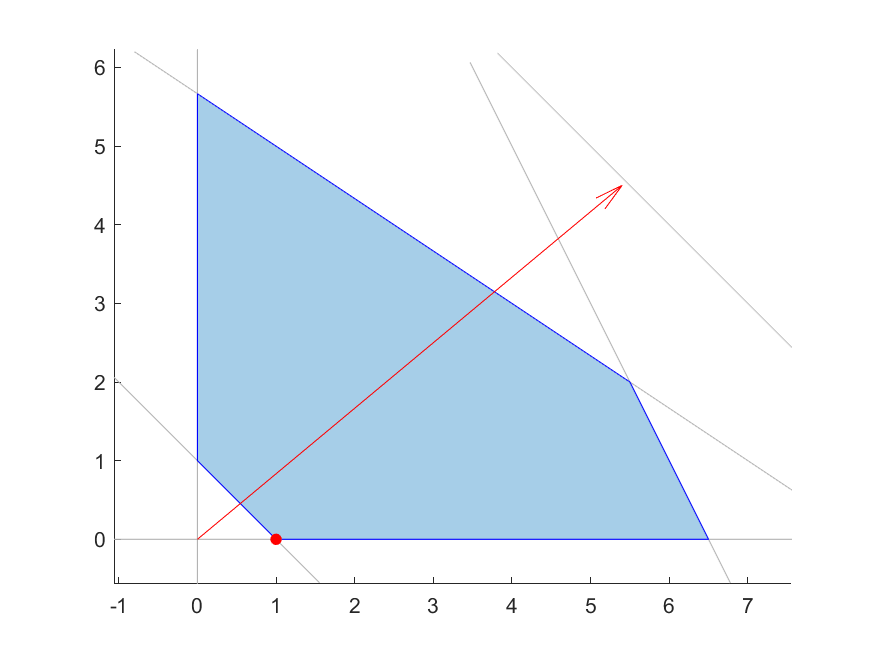
\includegraphics[width = \textwidth]{images/paper_simplex_point_1.png}
	\end{minipage}

	\vspace{6pt}
	\begin{minipage}{0.6\textwidth}
		\begin{align*}
		\begin{bmatrix}
		Z	& x		& y		& s_1	& s_2	& s_3	& s_4	& b \\
		1	& 0		& \textbf{2}		& 0		& 0		& -3	& 0		& -39 \\
		0	& 0		& 1/2	& 1		& 0		& -1/2	& 0		& 7/2 \\
		0	& 0		& \textbf{2}		& 0		& 1		& -1	& 0		& 4 \\
		0	& 0		& -1/2	& 0		& 0		& 1/2	& 1		& 11/2 \\
		0	& 1		& 1/2	& 0		& 0		& 1/2	& 0		& 13/2
		\end{bmatrix}
		\end{align*}
	\end{minipage} \hfill
	\begin{minipage}{0.35\textwidth}
		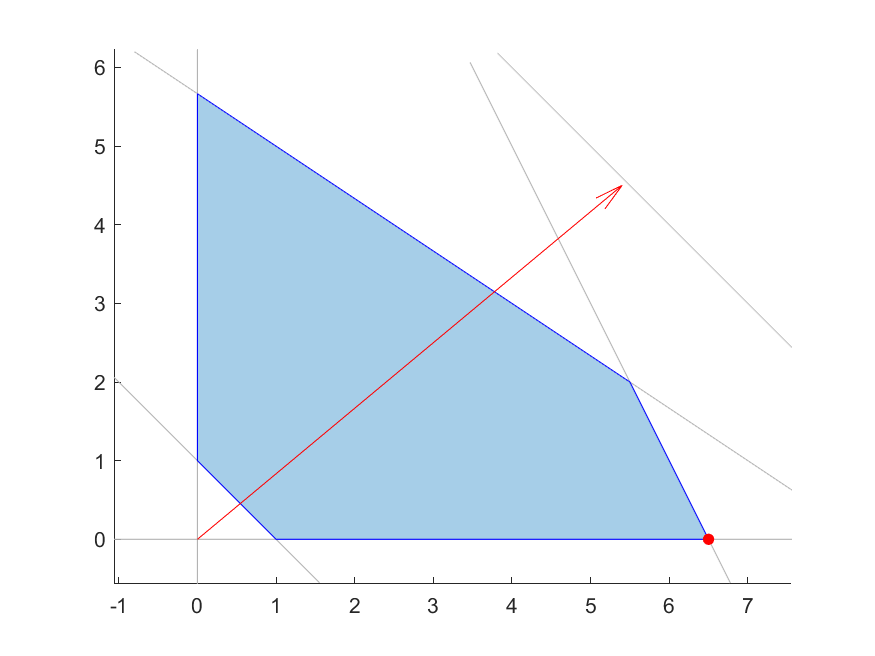
\includegraphics[width = \textwidth]{images/paper_simplex_point_2.png}
	\end{minipage}

	\vspace{6pt}
	\begin{minipage}{0.6\textwidth}
		\begin{align*}
		\begin{bmatrix}
		Z	& x		& y		& s_1	& s_2	& s_3	& s_4	& b \\
		1	& 0		& 0		& 0		& -1	& -2	& 0		& -43 \\
		0	& 0		& 0		& 1		& -1/4	& -1/4	& 0		& 5/2 \\
		0	& 0		& 1		& 0		& 1/2	& -1/2	& 0		& 2 \\
		0	& 0		& 0		& 0		& 1/4	& 1/4	& 1		& 13/2 \\
		0	& 1		& 0		& 0		& -1/4	& 3/4	& 0		& 11/2
		\end{bmatrix}
		\end{align*}
	\end{minipage} \hfill
	\begin{minipage}{0.35\textwidth}
		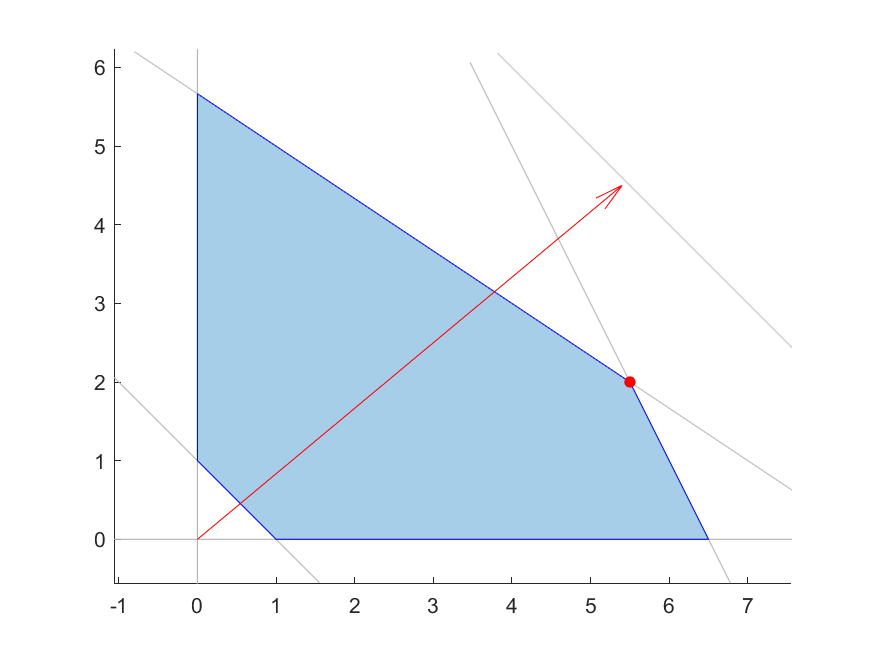
\includegraphics[width = \textwidth]{images/paper_simplex_point_3.png}
	\end{minipage}

	\vspace{6pt}
	The end result is $x=11/2 = 5.5, y = 2$, giving the farmer a total profit of \$43,000.
	
\end{answerblock}
\subsection{Efficiency and Uses}
The simplex algorithm is fairly efficient, and on average is polynomial time in the number of dimensions.\cite{schrijver} We can see that the algorithm cannot do better than polynomial time quite simply, by noting that for a single pivot operation in $n$ dimensions with $m$ inequality constraints, we require 1 row division for the leaving row, followed by $m$ row multiplications and additions to make the entering variable a basic variable. Assuming each of multiplication and division are constant time per element, this gives a total of $n+m+2 + 2m(n+m+2) = (2m+1)(n+m+2)$ operations per pivot, which is polynomial in the number of dimensions / constraints.
\begin{remark}
	By using a mechanism called the \textbf{dual problem}, an equivalent problem can be constructed that has $m$ variables and $n$ constraints, so distinguishing between them is not particularly useful in this analysis.
\end{remark}
However, it is the number of pivot operations needed that causes issues in complexity analysis. Presented above is one of the simplest rules for selection of entering and leaving variables (this is Bland's rule for entering\cite{bland}). This rule is quite inefficient in practice\cite{bernd-bland}, and other rules with much better performance exist, such as the Devex rule\cite{devex}. In general, the simplex algorithm requires a number of pivots cubic in the number of dimensions\cite{borgwardt}. However, it was shown by Klee and Minty that there is an infinite family of problems for which the simplex algorithm visits each of the $2^n$ vertices before terminating under the standard selection rules\cite{klee-minty}. In $n$ dimensions, the Klee-Minty cube is the linear programming problem\\
\begin{tabularx}{\textwidth}{X l l l X}
	& maximize		& $\sum_{i=1}^{n}2^{n-i}x_i$ & & \\
	& subject to	& $(\sum_{i=1}^{k}2^{k-i+1}x_i) - x_k \leq 5^k$ & $k=1,...,n$ &\\
	& 				& $x_k\geq 0$ & $k=1,...,n$ & 
\end{tabularx}
\cite{klee-minty}
Since this was proven, it has been shown that for any selection rule, there is a family of problems on which the simplex algorithm visits every vertex. This means that the worst case performance of the simplex algorithm is exponential in the number of dimensions, but several subsequent analyses have shown that the problems on which the simplex algorithm performs very poorly are in some sense "rare". \cite{spielman}

It should also be noted that the simplex algorithm as shown above is very space inefficient \cite{morgan}, as many real-world problems have thousands or millions of variables and constraints\cite{gurobi-blue-yonder}, rather than the 3 or 4 we have shown. Furthermore, in most industry applications, the matrix is sparse, so in industry the actual algorithm used is the revised simplex algorithm\cite{morgan}, which stores a sparse and invertible representation of the nonbasic variables, which reduces both the required storage space and the computational overhead. 

The simplex algorithm is often used in applications where the variables in question are continuous, or are discrete but sufficiently large that a small error is acceptable (e.g. if one is planning the division of \$1,000,000,000 to military departments, treating every dollar discretely is probably unnecessary, and a continuous approximation will suffice).
\section{Mixed Integer Linear Programming}
\subsection{Introduction}
While many problems have convenient continuous approximations, many others do not. For example, in scheduling contexts, where each person being scheduled has a fixed amount of time that they can contribute, and they cannot be doing two things at once. In these instances, we require that some variables have values that are either integers, or sufficiently close to integer values that the error is truly negligible. However, this problem is significantly harder than LP, which is already not trivial. Fully integer linear programming is NP-complete (and so NP-hard). In fact, even fully integer satisfiability (finding a single point satisfying all of the constraints) is NP-complete, and the special case where the variables are constrained to be binary is one of Karp's 21 NP-complete problems (proof of NP-hardness is shown by Karp via reduction from boolean satisfiability, which is known to be NP-complete)\cite{karp,cook}.

For scale on how difficult these problems are, consider a scheduling problem assigning 10 people to 10 items. There are some constraints on how these assignments can occur and some objective function, but for the moment we are interested in the worst case performance. Using a na\"{i}ve implementation of this problem gives 100 binary variables, one per possible person-item assignment. If we brute-force checked every possible configuration with the world's fastest supercomputer (at time of writing the Summit supercomputer in the Oak Ridge National Laboratory), with 200 PFLOPS, and supposing that checking each potential assignment takes only one floating point operation, it would take over 200,000 years to complete. If we assume the fastest possible computer, checking one potential assignment each Planck time, this would take about 70 femtoseconds. However, if we increase the number of people and items to 15 each, for a total of 225 variables, then it would take over 92 quadrillion years. This is almost 7 million times the age of the universe.

This assumes that we are just attempting to brute force the computation, which is obviously not a very good way to do it. However, many of the best methods known to mathematicians currently devolve to brute force. As the problem is NP-complete, it's intractable to even verify a solution is optimal without checking each possible solution.

Here we discuss one of the techniques observed to have reasonable performance on real-world problems, known as branch-and-cut\cite{mitchell-bandc}. The exact operation of the branch-and-cut algorithm in commercial solvers is, unfortunately, a trade secret, so we discuss only the general technique.
\begin{remark}
	Note that MILP is not convex, as an affine combination of two integer solutions will give non-integer solutions, so the feasible space is not convex due to the integrality constraints.
\end{remark}
\subsection{Theory}
Mixed Integer Linear Programming problems take the form\\
\begin{tabularx}{0.9\textwidth}{X l l l X}
	& maximize		& $\c^T\x$ & & \\
	& subject to	& $A\x \leq \b{}$ & &\\
	& 				& $\x\geq 0$ & & \\
	&				& $x_i\in\mathbb{Z},$ & $i=1,...,p\leq n$
\end{tabularx}
The branch-and-cut technique is a combination of two simpler techniques, branch-and-bound and cutting planes\cite{mitchell-bandc}. Branch-and-bound increases the lower bound for the possible solution, and cutting planes decrease the upper bound. The lower bound is always initialized to $-\infty$, and the upper bound is set to the optimum for the relaxation of the problem. The relaxation is the linear programming problem obtained by simply ignoring the integrality constraints. Any solution satisfying the integrality constraints is going to be no better than the optimum for the relaxation.
\subsubsection{Branch and bound}
The branch-and-bound technique explained here takes inspiration from binary search algorithms, and goes as follows\cite{land-doig-bnb}:
\begin{enumerate}
	\item Push the relaxation of the MILP problem to the queue.
	\item Loop until the queue is empty:\begin{enumerate}
		\item Take a problem from the queue, and solve. 
		\item If the value of this problem is equal to the current upper bound, then return and exit.
		\item If the value of this problem is worse than the current lower bound, discard this problem, then continue to the next loop.
		\item Otherwise, if the solution for this problem satisfies the integrality constraint, store this solution, and set the current lower bound to the value for this problem, then continue to the next loop.
		\item Otherwise (noting the solution is better than the current lower bound, but doesn't satisfy the integrality constraint), take one of the variables that should be integral, but isn't. Call this variable $x$ and its value in the solution to this problem $x'$, then create two new problems, one with $x\geq \lceil x'\rceil$, and one with $x\leq \lfloor x'\rfloor$ and push them to the queue.
	\end{enumerate}
\end{enumerate}
\subsubsection{Cutting planes}
The cutting planes method improves on the best known upper bound, by creating an additional linear constraint that removes the current solution without removing any potential integer solutions. In so doing, it removes whichever point previously produced the best result, forcing the solver to find a different point. This point should be slightly worse than the last point, thus the upper bound can be adjusted downward. If the solver ever finds an integer point by chance, then return that result, as that is guaranteed to be an integer point maximizing the MILP problem.

The cuts used are called Gomory cuts, and they were designed for fully integer problems. The adaptation to mixed integer problems is complex at best, and does not lend itself to intuitive understanding, so they will not be deeply explored here. For further information, see \cite{marchand-cp}
\subsubsection{Branch and Cut}
As the name implies, this is a combination of branch-and-bound and cutting plane techniques. This combination technique runs some number of cutting planes on the problem in step 2(a) of the branch-and-bound algorithm. It also runs some cutting planes on the top-level LP relaxation to improve the upper bound of the integer solution.

As already mentioned, the best methods of balancing these techniques are industry secrets, so a thorough explanation cannot be done here. It should, however, be noted that branch-and-bound devolves to brute force\cite{pataki-comp-bnb}, and cutting planes are not particularly effective in finding solutions in and of themselves, but tend to make branch-and-bound better. This shows that even the best known techniques are very difficult.
\subsection{Uses}
MILP is particularly useful in preference-based scheduling contexts, as the preferences can be continuous, but the schedules themselves are discrete\cite{gurobi-bbl-cs}\cite{gurobi-nfl-cs}. Other logistical decision problems are also easily translated to MILP problems\cite{gurobi-ppo-cs}, so MILP solvers are very useful.

As MILP is NP-complete, all other NP problems can be converted to a MILP problem in polynomial time, including some well known problems like the knapsack problem and the travelling salesman problem\cite{karp}.
\section{Quadratic Programming}
\subsection{Introduction}
Quadratic programming is a type of convex optimization that generalizes linear programming slightly. It allows the objective function to be a convex quadratic function, although the constraint functions still must be affine functions. This is useful as it allows for types of optimization like ordinary least squares, as well as for optimizing the variance of a random variable (which often arises in portfolio optimization)\cite{boyd}.
\subsection{Theory}
The objective function $f$ is permitted to take the form $f(\x) = \x^TQ\x + \c^T\x$, where this function is convex. On this type of function, requiring $f$ to be convex is equivalent to requiring $Q$ to be positive semidefinite.\cite{jorge-numopt}
\begin{theorem}
	$f(x) = \x^TQ\x + \c^T\x$ is convex if and only if $Q$ is positive semidefinite.
\end{theorem}
\begin{proof}
	Suppose $f$ is convex, then for any $\x_1,\x_2\in\R[n], a\in[0,1]$:
	\[
	f(\affcomb{\x_1}{\x_2}) \leq \affcomb{f(\x_1)}{f(\x_2)}
	\]
	Consider the left hand side. We see
	\begin{align*}
		LHS &= f(\affcomb{\x_1}{\x_2})\\
		&= (\affcomb{\x_1}{\x_2})^TQ(\affcomb{\x_1}{\x_2}) + \c^T(\affcomb{\x_1}{\x_2})\\
		&= a^2\x_1^TQ\x_1 + 2a(1-a)\x_1^TQ\x_2 + (1-a)^2\x_2^TQ\x_2 + a\c^T\x_1 + (1-a)\c^T\x_2
	\end{align*}
	On the right hand side, we see
	\begin{align*}
		RHS &= \affcomb{f(\x_1)}{f(\x_2)}\\
		&= a\x_1^TQ\x_1 + (1-a)\x_2^TQ\x_2 + a\c^T\x_1 + (1-a)\c^T\x_2
	\end{align*}
	As we had $LHS \leq RHS$, it must be the case that $RHS-LHS \geq 0$. Therefore, 
	\[
		a(1-a)\left[\x_1^TQ\x_1 - 2\x_1^TTQ\x_2 + \x_2^TQ\x_2\right]\geq 0
	\]
	This is trivially true for $a =0, 1$. Now supposing $a\in(0,1)$, 
	\begin{align*}
		\x_1^TQ\x_1 - 2\x_1^TTQ\x_2 + \x_2^TQ\x_2&\geq 0\\
		(\x_1-\x_2)^TQ(\x_1-\x_2)&\geq 0
	\end{align*}
	As $\x_1$ and $\x_2$ were arbitrary vectors, $\x_1-\x_2$ can be any vector in $\R[n]$, so $Q$ must be positive semidefinite. 
	
	Now suppose $Q$ is positive semidefinite. Then for any vector $\x\in\R[n]$, $\x^TQ\x\geq 0$. Take $\x_1,\x_2\in\R[n]$ such that $\x=\x_1-\x_2$. Then $(\x_1-\x_2)^TQ(\x_1-\x_2)\geq 0$. Take any $a\in[0,1]$. As $a(1-a)\geq 0$, we obtain that \[
		a(1-a)\left[\x_1^TQ\x_1 - 2\x_1^TTQ\x_2 + \x_2^TQ\x_2\right]\geq 0
	\]
	To each side of this inequality, add $a^2\x_1^TQ\x_1 + 2a(1-a)\x_1^TQ\x_2 + (1-a)^2\x_2^TQ\x_2 + a\c^T\x_1 + (1-a)\c^T\x_2$. This then gives that the left hand side is $a\x_1^TQ\x_1 + (1-a)\x_2^TQ\x_2 + a\c^T\x_1 + (1-a)\c^T\x_2$, or equivalently $\affcomb{f(\x_1)}{f(\x_2)}$. The right hand side is then $a^2\x_1^TQ\x_1 + 2a(1-a)\x_1^TQ\x_2 + (1-a)^2\x_2^TQ\x_2 + a\c^T\x_1 + (1-a)\c^T\x_2$, or equivalently $f(\affcomb{\x_1}{\x_2})$. So we then have that $\affcomb{f(\x_1)}{f(\x_2)}\geq f(\affcomb{\x_1}{\x_2})$, so $f$ is convex.
\end{proof}
There exist algorithms that solve QP problems in polynomial time when $Q$ is positive definite\cite{kozlov-comp-qp}, but if $Q$ is not positive definite then solving this problem is NP-hard\cite{sahni}.
\subsection{Quadratically Constrained Quadratic Programming}
Quadratically constrained quadratic programming is a further generalization of quadratic programming that allows the constraint functions to also be convex quadratic functions.\cite{boyd} This is also widely used in statistical applications, as it often occurs that one wants to maximize the expectation of some random variable, while limiting the maximum variance. As an example, suppose you are trying to optimize your investment portfolio. You have $n$ different stocks to choose from, where the current status of the stocks is given by the random variable $\vec{p}\in\R[n]$, which has known mean $\bar{p}$ and covariance $\Sigma$. The random variable $p$ is scaled to its present value, so that $p_i$ represents the price of stock $i$ at some fixed point in the future divided by its price now. Let $x_i$ denote the amount you invest in stock $i$, $B$ your total investment budget, and $\sigma_{max}$ the maximum risk you're willing to accept. Finally, suppose you don't want to short any stocks (equivalent to investing a negative amount in a stock). Then you can phrase the problem of maximizing your expected return subject to this maximum risk and budget as follows\cite{boyd}:
\begin{tabularx}{\textwidth}{X l l l X}
	& minimize		& $-\bar{p}^T\x$ & & \\
	& subject to	& $\x^T\Sigma\x-\sigma_{max}\leq 0$ & &\\
	& 				& $\vec{1}^T\x\leq B$ & & \\
	&				& $\vec{x}\geq 0$ & &
\end{tabularx}
\section{More Complex Convex Programs}
\subsection{Second-Order Cone Programming}
\subsubsection{Introduction}
Second-order cone programming sets the feasible space to be a second-order cone, but in effect it generalizes QCQP programs by allowing the matrices used to have a single negative eigenvalue, rather than forcing all of the eigenvalues to be greater than or equal to zero. This allows for limiting distances by another variable, which is often useful in engineering and space planning applications.
\subsubsection{Theory}
As stated above, the feasible space is a second-order cone, which is generally denoted as a set in $\R[n+1], S = \{(\x,t)|\lVert\x\rVert_2\leq t\}$, or equivalently \[ S=\left\{\begin{bmatrix}\x\\t\end{bmatrix}| \begin{bmatrix}\x\\t\end{bmatrix}^T\begin{bmatrix}I_n & \vz{n}\\\vz{n}^T & -1\end{bmatrix}\begin{bmatrix}\x\\t\end{bmatrix}\leq 0, t\geq 0\right\}\]\cite{boyd}. It can clearly be seen that the matrix in this constraint is not positive semidefinite, as the eigenvalue for the eigenvector with $\x=\vz{n},t=1$ is -1. However, with the addition of the condition $t\geq 0$, this is a convex set. \cite{boyd}
\subsection{Geometric Programming}
\subsubsection{Introduction}
\begin{definition}
	A \textbf{monomial} in the context of geometric programming is a function $f:\R[n]_{++}\to\R$, defined as $\x\mapsto cx_1^{a_1}x_2^{a_2}...x_n^{a_n}, c>0$.
\end{definition}
\begin{definition}
	A \textbf{posynomial} is any sum of monomials as defined above.
\end{definition}
A geometric programming problem takes the form \\
\begin{tabularx}{\textwidth}{X l l l X}
	& minimize		& $f_0(\x)$ & & \\
	& subject to	& $f_i(\x) \leq 1,$ & $i=1,...,p$ &\\
	& 				& $g_i(\x) = 1,$ & $i=1,...,q$ & 
\end{tabularx}
where $f_i$ are posynomials, and $g_i$ are monomials.\cite{duffin}\cite{boyd-gp} \\
These problems are actually not generally convex, but they are what is called log-log-convex\cite{boyd-dgp}, which is to say that if you substitute every variable for its logarithm, and take the logarithm of the objective function and the constraint functions, then the resulting problem is convex, and corresponds uniquely to the original problem.

These types of problems often arise in integrated circuit design\cite{boyd-gp-opamp}, where the volumes and areas of various components need to be optimized, while keeping solid connections with sufficient cross sectional area for current flow, etc. All of those constraints involve muliplying several variables together, and possibly adding those products together, perfectly suited to the above description of monomials and posynomials.
\subsubsection{Theory}
As mentioned above, these problems can be converted to convex problems by substituting the variables for their logarithms and taking the logarithms of the functions. Consider first a monomial $g(\x) = cx_1^{a_1}x_2^{a_2}...x_n^{a_n} = \exp(\log(c) + a_1\log(x_1) + a_2\log(x_2) + ... + a_n\log(x_n))$. Substituting $y_i = \log(x_i)$ gives $g'(\vec{y}) = \exp(\log(c) + a_1y_1 + a_2y_2 + ... + a_ny_n)$, then taking the logarithm of this gives $\tilde{g}(\vec{y}) = \a^T\vec{y} + \log(c)$. As we had that $g_i(\x) = 1$, we have that $\tilde{g}(\vec{y}) = 0$. For the posynomials, this is slightly more complex. Consider $f(\x) = \sum_{i=1}^{p}c_i\prod_{j=1}^{n}x_j^{a_{ij}}$. By substituting $y_i = \log(x_i)$, we get $f'(\vec{y})=\sum_{i=1}^{p}\exp\left(\log(c_i) + \sum_{j=1}^{n}a_{ij}y_j\right)$. Taking the logarithm, we obtain $\tilde{f}(\vec{y}) = \log\left(\sum_{i=1}^{p}\exp\left(\log(c_i) + \sum_{j=1}^{n}a_{ij}y_j\right)\right)$. This is the composition of a function called log-sum-exp with an affine function. As noted by Boyd, \cite{boyd} this is also a convex function if log-sum-exp is convex.
\begin{theorem}
	$f(x) = \log\left(\sum_{i=1}\exp(x_i)\right)$ is a convex function.
\end{theorem}
\begin{proof}
	Take $\x, \vec{y}\in \R[n]$. Then take $u_i = \exp(x_i), v_i = \exp(y_i), a\in[0,1]$. Then $f(\affcomb{\x}{\vec{y}}) = \log\left(\sum_{i=1}^{n}u_i^av_i^{(1-a)}\right)$. Then by H\"{o}lder's inequality, as $u_i, v_i>0$ we have that $\sum_{i=1}^{n}u_i^av_i^{(1-a)} \leq (\sum_{i=1}^{n}u_i^{a\frac{1}{a}})^a(\sum_{i=1}^{n}v_i^{(1-a)\frac{1}{1-a}})^{(1-a)}$, so then we have that $\log\left(\sum_{i=1}^{n}u_i^av_i^{(1-a)}\right)\leq a\log\left(\sum_{i=1}^{n}u_i\right) + (1-a)\log\left(\sum_{i=1}^{n}v_i\right)$, or equivalently that $f(\affcomb{\x}{\vec{y}})\leq\affcomb{f(\x)}{f(\vec{y})}$.
\end{proof}
Then as log-sum-exp is convex, and the function $\tilde{f}$ is the composition of log-sum-exp and an affine mapping, $\tilde{f}$ is convex. Once this transformation is performed, the problem can be solved much more easily, then transforming back is straightforward as well, using $x_i = \exp(y_i)$.
\subsection{Semidefinite Programming}
\subsubsection{Introduction}
	Semidefinite programming is one of the most general kinds of convex optimization, encompassing LP, QP, QCQP, and SOCP. Many other optimization problems can be well approximated by semidefinite programming problems. In fact, semidefinite programming is so general that many commercial solvers that solve all of the above problems actually convert them first to an SDP problem, then solve that SDP problem.
\subsubsection{Theory}
	\begin{definition}
		Given a $n\times n$ matrix $A$, $\textrm{tr}(A)$ is the sum of the diagonal elements of $A$. 
	\end{definition}
	\begin{definition}
		Given two symmetric $n\times n$ matrices $A, B\in\mathbb{S}^n$, define $\langle A,B\rangle_{\mathbb{S}^n} = \textrm{tr}(A^TB)$, where $\mathbb{S}^n$ represents the space of all symmetric $n\times n$ matrices.
	\end{definition}
	Semidefinite programming problems take the following form\\
	\begin{tabularx}{\textwidth}{X l l l X}
		& minimize		& $\langle C,X\rangle_{\mathbb{S}^n}$ & & \\
		& subject to	& $\langle A_k,X\rangle_{\mathbb{S}^n}\leq b_k,$ & $k=1,...,m$ &\\
		& 				& $X\succeq0$ & & 
	\end{tabularx}
	where $A_k, C, X\in\mathbb{S}^n$, and $X\succeq0$ means $X$ is positive semidefinite\cite{freund}. This actually encapsulates polynomial constraints as well. This comes in with the constraint of positive semidefiniteness for $X$. This constrains its eigenvalues to all be positive. As the eigenvalues are solutions to the characteristic equation $|X-\lambda I|=0$, this constrains the $n$-th order polynomial to only have positive solutions, which is sufficient to have polynomial constraints of order less than $n$.
\subsection{Closing Comments On Convex Optimization}
	For most of these types of optimization, we did not go into much detail, touching only on their representation and some vague techniques for problem conversions and solutions. That is because for most applications, LP and MILP will be sufficient for the beginning optimizer, and as the advanced solving techniques become significantly more complex in presumed background, they tend to confuse more than enlighten. It is worth noting again that all of these different techniques because you should always use the least complicated model that encapsulates all of the necessary information, as using a more complex model makes it significantly harder to solve.
\section{An Example of Non-Convex Optimization}
\subsection{Introduction}
	While many problems can be expressed as a convex optimization problem, or can be converted to an equivalent convex optimization problem, there are many other problems that cannot. This is especially the case in many engineering problems, where even if the problem itself were technically convex, finding a closed form for the feasible region or the objective function is nigh on impossible. One specific example of this is 3D modelling, where mechanical engineers want to have a program design a mechanical part fitting some parameters, and optimize its performance under certain circumstances, as evaluated by a simulation. This is referred to as \textbf{black-box optimization}, which is where the objective function is a black box. In all previous algorithms discussed, the algorithm has information about the objective function that it can use in optimizing. In black-box optimization, the algorithm can only give inputs to the objective function, and the function gives back a singular value. This makes the problem significantly harder. In this particular case, evaluations of the objective function are also expensive, both in terms of resources and time, so we want to find our optimum with as few evaluations of the objective function as possible. Finally, we would like to find a global optimum, even though our objective function may not be convex (recall that the reason convex optimization is used is because all local optima are also global optima). Given the information we have from convex optimization, this seems like an impossible task, but algorithms do exist with reasonable performance on problems of exactly this type.
\subsection{Mode-Pursuing Sampling}
	The problem we are attempting to optimize is \\
	\begin{tabularx}{\textwidth}{X l l l X}
		& minimize		& $f(\x)$ & & \\
		& subject to	& $\x\in S(f)\subset\mathbb{R}^n$ & &
	\end{tabularx} 
	where $S(f)$ is a compact set. The paper we reference uses the simplifying supposition that $S(f) = [a,b]^n$ for some known $-\infty<a<b<\infty$, and we do the same here.
	The method we will be discussing is the method proposed by Liqun Wang, Songqing Shan, and G Wang in Mode-Pursuing Sampling Method for Global Optimization on Expensive Black-box Functions\cite{wang-mps}. The proposed method begins with a method called the mode-pursuing sampling algorithm, which clusters sampled points around the mode of an arbitrary probability density function. It begins with a modification of a sampling algorithm provided by Fu and Wang\cite{fu-sampling}, which is summarized very well in the paper, and so will not be again summarized here. For the purposes of this analysis, it suffices to know that the method generates a discrete probability distribution from a given continuous probability density function, which approximates the initial PDF asymptotically well as the number of sampled points increases. 
	
	The mode-pursuing sampling algorithm uses this samplying in a 4 step loop, where $P_s$ is the set of sampled points and the function's value at those points. There are two observations that should be made first though; 1. minimizing $f$ is, as with convex optimization, the same as maximizing $-f$, and 2. Either $f$ is unbounded below on $S(f)$, or there exists some $c$ such that $f(\x)\geq c\forall\x\in S(f)$, so $f$ is assumed to be positive on $S(f)$ without loss of generality, as either a constant may be added to make that true, or there is no solution anyway.
	\begin{enumerate}
		\item Generate a starting set of $m$ initial points $x^{(1)},x^{(2)},...,x^{(m)}$ distributed uniformly on $S(f)$. Add these points and their function values to $P_s$.
		\item Use all of the points and function values in $P_s$ to generate a continuous approximation $\hat{f}$ to $f$ such that $\hat{f}(\x^(i)) = f(\x^{(i)})$ for each $\x^{(i)}\in P_s$.
		\item Define $g(\x) = c_0 - \hat{f}(\x)$, where $c_0$ is any constant such that $c_0 \geq \hat{f}(x)\forall\x\in S(f)$. This makes $g$ a probability density function, up to some normalizing constant. The most probable points are the points close to the maxima of $g$, which occur at the minima of $\hat{f}$. Use Fu and Wang's sampling method to sample $m$ more points according to $g$.
		\item Add the newly generated points and their function values to $P_s$. If some stopping criterion is met, then exit with the best answer so far, otherwise go to step 2.
	\end{enumerate}
	In step 2, the authors use a linear spline function, for reasons detailed in their paper. While these reasons are interesting, they are a bit too in-depth for this analysis, so here we will simply note that they generate an approximation that works well for this algorithm.
	
	This method is quite nice in its relative simplicity, as they note that if no stopping criterion is applied then this algorithm converges to the true optimum of $f$, and by construction it ensures that it continues to sample the global function even as it approaches the minimum around the current mode, so it ensures that it does not miss the global optimum while exploring near a local optimum.
	
\subsection{Global Optimization Strategy}
	While we have already expressed that the algorithm so far is reasonable, and converges to the optimum eventually, as described it can be quite slow to converge, especially if the objective function is relatively flat around the global optimum. To address this, the authors introduce two items. One switches the algorithm to a local search mode if a certain criterion is met, and the other is referred to as a speed control factor. We explore the local search mode first.
	
	The authors note that any smooth function can be locally and accurately approximated by a quadratic function (by Taylor's Theorem). They suppose that if the best quadratic approximation around the current mode then it is a reasonable indicator that the current mode is near the global optimum. Using a quadratic approximation of the objective function makes optimizing in a local area trivial. If the neighbourhood of the current best mode does not well fit a quadratic model, then the algorithm emphasizes searching the rest of the space, hoping to find a mode that is better approximated by a quadratic model. If the current mode does fit a quadratic model sufficiently well, then the algorithm performs inexpensive quadratic optimization to find its minimum. If that minimum is sufficiently close, then the algorithm returns that minimum, otherwise it again emphasizes searching the rest of the space. 
	
	The way that the algorithm controls whether it explores near the current mode or emphasizes the rest of the search space is using the speed control factor. It modifies the functioning of Fu and Wang's sampling method, to make the current modes more or less probable, and the surrounding area correspondingly less or more probable.
	
	By using these mechanisms, the algorithm converges to a value significantly quicker, but it also has a much higher probability of getting stuck on, or returning the value of, a local minimum rather than the global minimum, as the emphasis on local searching makes it significantly easier to overlook the global minimum.
\subsection{Closing comments on non-convex optimization}
	I, personally, think this is quite an ingenious method of optimization. That said, although the authors report that it is effective even on functions for which the objective function is convex, previously known, or not expensive, the detriments of potentially returning a local minimum instead of the desired global minimum are reason enough to stick with well established solutions when they work. The method as described in this paper also does not allow for mixed integer optimization, although some of the authors have continued working on variants of this method, including methods accommodating discrete variables\cite{mps-dv}.
	
	Non-convex optimization is generally about balancing the time spent searching for a solution with minimizing the risk of getting the wrong answer, and I think this method does rather well at that.
\section{Conclusion}
	We have discussed many different types of optimization, primarily convex optimization, and with an emphasis on linear programming. At this point I want to note again that for most real-world problems, a mixed-integer linear program is more than sufficient to approximate the problem, so explaining linear programming and mixed integer linear programming in greater detail is likely to prove more beneficial to the future optimizer than explaining the general optimization subclasses in significantly more detail than presented here. To those whose interest in these classes has been piqued, the textbook Convex Optimization by Stephen Boyd and Lieven Vandenberghe is a fantastic resource for further reading, especially on the theory. However, in this paper I have provided an overview of some of the most common or interesting items in mathematical optimization, balancing mathematical rigour and ease of comprehension.
\printbibliography
\end{document}
